%
% File dialogue-2022.tex
%
% Made by Serge Sharoff following the style guide file for COLING-2020,
% see the full story in https://coling2020.org/coling2020.zip

\documentclass[11pt]{article}

\usepackage{dialogue}

\usepackage{ifxetex}
\ifxetex
    \usepackage{fontspec}
    \setromanfont{Times New Roman}
\else
  \usepackage{cmap}
  \usepackage[T2A,T1]{fontenc}
  \usepackage[utf8]{inputenc}
  \usepackage{times}
  \usepackage{latexsym}
  \usepackage{substitutefont}
  \substitutefont{T2A}{\familydefault}{cmr}
\fi

% \usepackage{subfig}
\usepackage{caption}
\usepackage{subcaption}

\usepackage[russian,british]{babel}
\usepackage{url}
\usepackage{pgf}

%% For proper formatting of linguistic examples use
%% https://anorien.csc.warwick.ac.uk/mirrors/CTAN/macros/latex/contrib/covington/covington.pdf
\usepackage{covington} %% comment it out if you do not require this option

%% To make citations and references clickable
\usepackage{hyperref}

\renewcommand{\ttdefault}{lmtt}

\dialogfinalcopy % Uncomment this line for the final submission
\newcommand{\score}[2]{$#1\  \scriptstyle \pm #2$}
\newcommand{\bestscore}[2]{$\textbf{#1}\  \scriptstyle \pm #2$}

\title{Controllable Multi-attribute Dialog Generation with PALs and Grounding Knowledge}

\author{Evseev D. A. \\
  Moscow Institute of Physics \\
  and Technology \\
  Dolgoprudny, Russia \\
  {\tt dmitrij.euseew@yandex.ru} \And
  Nagovitsin M. S. \\
  Moscow Institute of Physics \\
  and Technology \\
  Dolgoprudny, Russia \\
  {\tt nagovitsin.ms@phystech.edu}
  \AND
  {\bf Kuznetsov D. P.} \\
  Moscow Institute of Physics and Technology \\
  Dolgoprudny, Russia \\
  {\tt kuznetsov.dp@phystech.edu} \\
  }

\date{}

\begin{document}
\maketitle
\begin{abstract}
Today, neural language models are commonly employed for generation of natural like responses in dialog systems. The main issue that limits wide adoption of neural generation is related to poor predictability of responses in terms of content, as well as dialog attributes such as dialog acts and sentiment.
%Controllable generative models have an ability to output responses for particular attributes (e.g. dialog act or sentiment) or with a particular content. 
In this paper we propose a method based on projected attention layers (PALs) for controllable multi-attribute knowledge grounded dialog generation. We compared a number of methods for training and blending representations produced by PALs combined with DialoGPT base model. Results of our experiments demonstrate that separate pre-training of PAL branches for different attributes followed by transfer and fine-tuning of dense blending layer gives the highest accuracy of control of a generated response for fewer trainable parameters per an attribute. Furthermore, we applied our approach for controllable multi-attribute generation with grounding knowledge to Blenderbot model. Our solution outperforms the baseline Blenderbot and CRAYON model in control accuracy of dialog acts and sentiment on Daily Dialog as well demonstrates a comparable overall quality  of dialog generation given grounding knowledge on Wizard of Wikipedia.
  
\textbf{Keywords:} controllable dialog generation, knowledge grounded dialog generation, projected attention layers.

\textbf{DOI:} 10.28995/2075-7182-2022-20-XX-XX
\end{abstract}

\selectlanguage{russian}
\begin{center}
  \russiantitle{Управляемые диалоговые генеративные модели с параметризацией атрибутов и дополнительным контекстом генерируемых реплик на основе PALs}

  \medskip \setlength\tabcolsep{1cm}
  \begin{tabular}{cc}
    \textbf{Евсеев Д. А.} & \textbf{Наговицин М. С.}\\
      Московский физико-технический & Московский физико-технический\\
      институт & институт \\
      Долгопрудный, Россия & Долгопрудный, Россия\\
      {\tt dmitrij.euseew@yandex.ru} & {\tt nagovitsin.ms@phystech.edu}
  \end{tabular}
  \begin{tabular}{c}
    \textbf{Кузнецов Д. П.}\\
      Московский физико-технический институт\\
      Долгопрудный, Россия\\
      {\tt kuznetsov.dp@phystech.edu}
  \end{tabular}
  \medskip
\end{center}

\begin{abstract}
В настоящее время нейронные языковые модели широко используются для генерации реплик в диалоговых системах. Основной недостаток нейронной генерации связан с непредсказуемостью содержания реплик. В данной статье мы предлагаем метод, основанный на проекционных слоях внимания (PAL) для управления несколькими параметрами генерируемой реплики. Мы сравниваем несколько методов обучения и смешивания представлений, полученных с помощью PALs, добавленных к в DialoGPT. В ходе экспериментов было установлено, что обучение PALs отдельно для каждой из веток управляемых параметров и последующее дообучение полносвязного смешивающего слоя приводит к наибольшей точности управляемой генерации, при этом используя меньшее число обучаемых параметров. Также мы применили наш подход для генерации с контролем атрибутов опираясь на внешние знания, с помощью модели Blenderbot. Наше решение превосходит базовую версию Blenderbot и модель CRAYON по точности предсказания диалогового акта и сентимента генерируемых реплик на датасете Daily Dialog, и при этом показывает сравнимое качество генерации реплик с использованием контекста на датасете Wizard of Wikipedia.
  
  \textbf{Ключевые слова:} управляемая генерация реплик в диалоге, генерация реплик по контексту, проекционные слои внимания.
\end{abstract}
\selectlanguage{british}

\section{Introduction}
\label{intro}

Majority of open-domain dialog systems use hand-crafted finite state machines for response generation \cite{larsson2000information}, \cite{bocklisch2017rasa}, \cite{finch2020emora}. For every expected user utterance these systems define a state with a pre-defined output response and transition to the next state of the dialog, but user input can mismatch a condition for transition in the current state.  As well, the user input can mismatch all possible states defined by the finite state machine. Here, neural generative models can help with producing natural responses. Unfortunately, generative models demonstrate very unreliable coherence with existing dialog context \cite{abhishek2021transformer}. One of the possible solutions is to use controllable attributes such as dialog act or sentiment to guide a generation of responses and return the dialog flow to the domain of a pre-defined script. If the script is defined as pairs of adjacent dialog acts, or in goal-oriented dialog, the attributes of the system response (intent, slot values) are extracted \cite{wu-etal-2019-transferable}, for known attributes of the response a generative model conditioned on grounding knowledge about entities found in the dialog context or slot values, can generate all the bot utterances in the script without retrieval of hand-written responses. Also, the right level of control can improve dialog quality in different aspects \cite{see2019makes}. Social bots like Gunrock \cite{gunrock} and XiaoIce \cite{zhou2019design} are actively using dialog acts, sentiment, and other attributes for dialog management.

Controllable generative models have been an active area of research over the last few years. Models \cite{zhao2017learning}, \cite{zhang2018learning} control one attribute of the generated response (dialog act, response relatedness or specificity). The need to control different attributes simultaneously is present in \cite{see2019makes}. General approaches to control multiple attributes simultaneously were presented for different model architectures in \cite{hu2021controllable}, \cite{neural_meta_words}, \cite{attr_alignment}, \cite{side_control}, \cite{phed}. In this paper, we propose and study a technique for multi-attribute generation control which is suitable for both pre-training as well as fine-tuning. We use PALs \cite{stickland2019bert} with transformer architectures, consequently, parameters of the main pre-trained model provide constant background knowledge, and PAL layers are trained to control generation with respect to specific attribute.

Informativeness and meaningfulness is another important aspect of generated responses. Blenderbot \cite{roller2020recipes}, CoLV \cite{zhan2021colv} and CGRG \cite{wu2021controllable} use grounding knowledge (retrieved paragraphs) to control the content of output utterances. But these models are not able to be controlled to produce the response with required attributes, such as dialog act or sentiment.

Trained models for the English language, training and inference code and data to test the quality of models are published in Open Source under the Apache 2.0 license (anonymized link). The main contributions of this work are the following:
\begin{itemize}
    \item we develop the method of controllable generation for several simultaneous attributes such as dialog acts and sentiment with no changes in weights of the original model;
    \item we study simultaneous control of knowledge grounding as well as dialog act and sentiment of a response, and find that our model outperforms existing approaches in terms of dialog act and sentiment control accuracy and is competitive in terms of perplexity of knowledge grounded generation.
\end{itemize}

\section{Related Work}

% \subsection{Methods of controllable generation}
There are many different approaches to controlling the generation process with or without changing the architecture or retraining the initial language model. PPLM \cite{pplm} updates latent representations of the model during decoding with help of a pre-trained discriminator, GeDI \cite{gedi} uses class-conditional distributions to achieve control for both desired and undesired attributes (for example, generate less toxic answers). Both PPLM and GeDI work without changing the initial model. 

Another way of control is to add special control tokens as an input for the model. It can be done by fine-tuning (or full training) the model, as proposed in CTRL \cite{ctrl}, or by keeping the initial model as is and training a special alignment function that will generate proper key and value representations for control tokens on each level of pre-trained Transformer model, as proposed in Attribute Alignment \cite{attr_alignment}. Those methods are capable of controlling multiple attributes by adding tokens for each one.

For larger models prefix tuning \cite{prefix_tuning} can be applied. Prompts also can be used for a few shot learning \cite{prompt_based_few_shot}.

Some methods work with a latent space, for example, CRAYON \cite{hu2021controllable}, which is based on LSTM, or PHED \cite{phed}, which uses a Transformer combined with CVAE to add a latent space to the Transformer architecture. Model GTMES2S, proposed in \cite{neural_meta_words} uses additional modules to control the current level of all attributes and guide further generation to reach desired values. Each of CRAYON, PHED, and GTMES2S are working with multiple attributes. In XiaoIce dialog assistant \cite{zhou2019design} GRU is used to generate responses, conditioned on query and response empathy vectors.

The other method is to add special modules to shift embeddings (and maybe hidden states) from the initial model, same as with PPLM \cite{pplm}, but to learn proper transformations in advance and not to tune them on inference. SideControl \cite{side_control} proposes a way to perturb embeddings of any language model by training additional modules, which will take class embedding or grounding knowledge into account. Another way is to treat control as a special task and add adapters \cite{houlsby2019parameterefficient} for different attributes we want to control. One of such models is Adapter-Bot \cite{madotto2020adapterbot} which has an option of switching between different attributes without changes in the initial model. Hyperformer \cite{mahabadi2021parameter} utilizes shared PAL parameters for all tasks and Transformer layers, these parameters are generated by a hypernetwork. The model \cite{xie2021empathetic} is an encoder-decoder Transformer, where emotions in response are controlled with emotion embeddings, which are fed into the model. But models with adapters are not able to control multiple attributes simultaneously without additional work. Task-specific parts to the model can also be efficiently added with help of low-rank decomposition, as proposed in LoRA \cite{lora}.

The key points in which our model differs from the others are the following:

\begin{itemize}
    \item Ability to control multiple attributes simultaneously (dialog act and sentiment in our study);
    \item Preserving the weights of the initial model in the original state;
    \item Ability to pre-train all adapters independently on different datasets;
    \item Scalability in terms of number of controllable attributes and number of their values;
\end{itemize}

Most generative models, which do not use external knowledge, are capable of producing grammatically correct and natural responses given the dialog history but have a limited ability to generate interesting responses based on facts. On the other hand, knowledge-grounded generative models have the option of controlling the content of generated responses with sentences with facts or keywords. CGRG \cite{wu2021controllable} model uses lexical control phrases to control the generated response. The approach of \cite{xu2021retrieval} is based on PALs for different topics which are used for retrieval-free knowledge grounded generation. The model \cite{zhan2021colv} uses latent variables for relevant knowledge selection and response generation. The models \cite{xu2021generating}, \cite{kumar2021controllable} and \cite{gupta2020controlling} controls the generated response by adding as input of the transformer the sequence of keywords before the dialog history. Our approach is inspired by Blenderbot \cite{roller2020recipes} which is an encoder-decoder transformer pre-trained on Reddit and finetuned on Wizard of Wikipedia \cite{dinan2018wizard}, but our model controls not only the content of the response but also dialog act and sentiment.

\section{Methods}
In this paper, our goal is to find a method to control different response attributes without losing much token prediction quality (perplexity) and other abilities of the base pre-trained model (e.g., using grounding knowledge). We did most of our experiments with   DialoGPT-small architecture \cite{zhang2020dialogpt}, because of the affordable time to fine tune and the good quality of the pre-trained model. 
Additional experiments with simultaneous control of content, dialog act, and sentiment we performed with Blenderbot architecture \cite{roller2020recipes}.
Furthermore, we chose dialog acts (inform, question, directive, commissive) and sentiment (negative, neutral, positive) as controlled attributes. For evaluation of control accuracy we used DailyDialogs \cite{li2017dailydialog}, sentiment labeling was made separately by a classifier. For evaluation of knowledge-grounded dialog generation quality (perplexity), we used Wizard of Wikipedia dataset \cite{dinan2018wizard}.

\begin{table*}[h]
\fontsize{9}{11}
\selectfont
\centering
\begin{tabular}{cccccccc}
\hline
Control     & Blend    & Train dataset & Dialog act acc. & Sentiment acc. & Perplexity & Opt. steps & Trainable par. \\ \hline
            % &          &  dataset   & accuracy & accuracy &    & steps & parameters \\ \hline
No control  & -        & DailyDialogs  & \score{25.20}{0.21}          & \score{33.41}{0.15}          & \bestscore{15.19}{1.58} & 2000 & 117M \\ 
Dialog acts & average     & DailyDialogs  & \bestscore{63.74}{0.32} & \score{42.83}{0.27}          & \score{15.93}{0.12} & 10000 & 36M \\ 
Dialog acts & dense & DailyDialogs  & \score{45.27}{5.26}          & \score{40.15}{1.22}          & \score{22.36}{0.85} & 5000 & 49M\\ 
% Dialog acts & dense x2 & DailyDialogs  & \score{50.12}{1.76}          & \score{41.78}{0.27}          & \score{18.84}{0.46}  & 5000 & 40M\\ 
Sentiment   & average     & ScenarioSA    & \score{33.40}{0.16}          & \bestscore{72.09}{4.06} & \score{92.98}{14.74}  & 5000 & 28M \\ \hline
\end{tabular}
\caption{Models with control of one attribute. The model with no control is a finetuned DialoGPT-small, models with control are DialoGPT-small with PALs. Metrics were calculated on valid set of Daily Dialog.}
\label{one_attribute_control}
\end{table*}

\begin{table*}[ht]
\fontsize{9}{11}
\selectfont 
\centering
\begin{tabular}{ccccccc}
\hline
Blend          & Transfer & Dialog act acc.  & Sentiment acc.   & Perplexity  & Opt. steps  & Trainable par. \\ \hline
average           & no       & \score{63.09}{2.22} & \score{69.19}{1.10} & \score{17.12}{0.40} & 5000 & 63M \\
dense          & no       & \score{61.65}{1.02} & \score{67.10}{1.38} & \score{22.07}{0.39} & 5000 & 84M \\
dense \& average & no       & \score{61.36}{1.40}  & \score{68.12}{0.69} & \score{15.51}{0.13} & 5000 & 77M \\
average           & yes      & \bestscore{65.62}{2.04} & \score{66.04}{0.25} & \score{17.74}{0.75} & 5000 & 63M \\
weighted average  & yes      & \score{63.20}{1.09} & \score{69.05}{0.42} & \score{15.65}{0.09} & 5000 & 63M \\
dense          & yes      & \score{60.83}{1.35} & \score{67.80}{3.37} & \score{21.34}{0.40} & 5000 & 84M \\
dense \& average & yes      & \score{62.76}{0.70} & \bestscore{70.03}{2.04} & \score{15.69}{0.19} & 5000 & 77M \\ 
dense \& average, only blend & yes      & \score{60.19}{0.76} & \score{67.47}{0.90} & \bestscore{15.30}{0.05} & 10000 & 14M \\ \hline
\end{tabular}
\caption{Models with simultaneous dialog act and sentiment control. Transfer averages that PALs were initialized with weights from model for single attribute control.}
\label{two_attributes_control}
\end{table*}

\subsection{Projected Attention Layers as Multitask Adapters}
One of the approaches to control object attributes is to learn proper shifts in latent space \cite{hu2021controllable}. One way to modify latent representations for every token is to use \textit{Projected Attention Layers (PALs)} \cite{stickland2019bert} as adapters for every controllable attribute. In our case, each PAL will learn to correct hidden states of the main model to generate a response with the desired attribute (Figure~\ref{adding_pals_dialogpt}).
% Idea: shifting of prediction like shifting in gradient boosting
% TODO: add block of cell for fig
\begin{figure}[ht!]
    \centering
    % 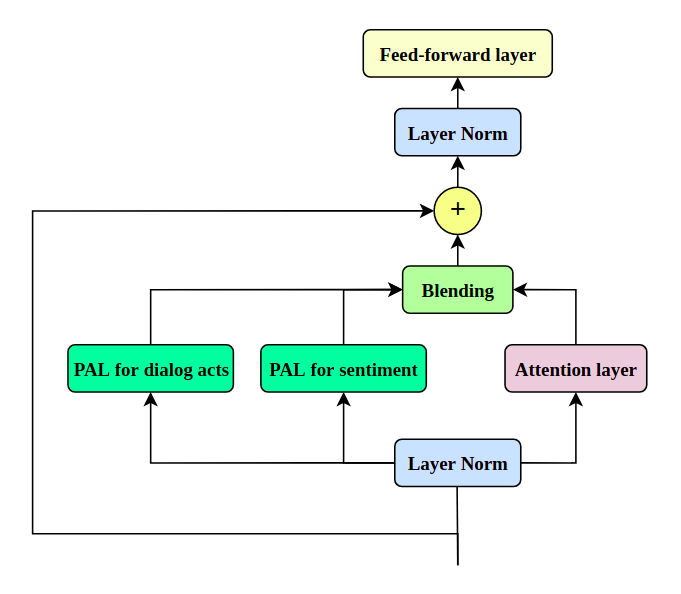
\includegraphics[width=0.48\textwidth]{img/pals_and_main.png}
    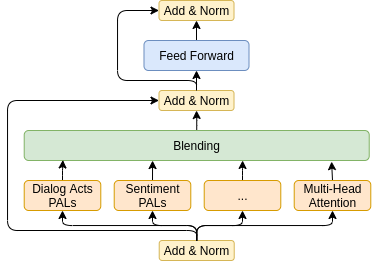
\includegraphics[width=0.5\textwidth]{img/pals_model.png}
    \caption{Blending of PALs and multi-head attention of Transformer hidden representations for every token.}
    \label{adding_pals_dialogpt}
\end{figure}

\subsection{Blend layer}
To control several attributes simultaneously, we decided to add a PAL for each attribute and run them in parallel (Figure~\ref{adding_pals_dialogpt}). 
%We can still just add all PAL's outputs to hidden states of the main model on each layer, but since we add an arbitrary number of PALs in parallel, the summation scales poorly. This is due to the inconsistency of absolute values of hidden states and their dependency on the number of attributes to control. For this reason, 
We chose \textit{average blending} as our baseline for blending hidden representations. It allows us to control easily the contribution of each PAL to the resulting hidden states by weighting them. Then we try a trainable way of blending outputs of PAL branches: \textit{dense blending} --- concatenation of PALs outputs and the main branch and feeding into the dense layer; \textit{combination of dense and average blending} --- concatenation of PALs outputs, feeding into the dense layer and averaging the output with the base model.
The loss function stays unchanged from the task of the next token prediction. For every labeled sample from training data we chose only corresponding PALs and train them, the base model is frozen. %For example, if the target utterance is a positive (sentiment) question (dialog act) then we turn on PAL for positive sentiment and PAL for question dialog act and train them. %Batching is obtained by grouping utterances with the same attributes.

\subsection{Default branch}
We added the \textit{"default" branch} for each attribute for default selection values for attributes. 
%If we use a blending layer without trainable parameters, we can try not to take the corresponding PAL into account, but for some blending layers, the number of input vectors is fixed. 
The default branch is turned on for training on every sample instead of specialized PAL with probability $p = 0.2$. Thus default branch will be trained on the entire dataset and will not be bound to one attribute value.

\subsection{Independent PALs pre-training}
We independently trained models for dialog act and sentiment control and transferred these pre-trained branches into one model. Even without any further training resulting model demonstrated a noticeably good attribute control without huge degradation of perplexity, even though PALs for the sentiment were trained on a different dataset (more details in Appendix ~\ref{sec:average_blending}). After transfer, the model with the blending layer can be finetuned on the target dataset. 
% Each architecture showed better control abilities without losing perplexity being trained with transferred weights.

\subsection{Control of attributes and context of responses}

One of our goals is to develop a model which could generate responses for a given grounding knowledge and global attributes, such as dialog act and sentiment. %Reddit corpus contains about 147M dialogs on different topics. dialogs in Wizard of Wikipedia dataset are discussions on Wikipedia pages, and some of the utterances in these dialogs can contain facts from one of the pages. In Blenderbot the inputs are dialog history and grounding knowledge, separated with a special token, and output is the response which can be based on grounding knowledge. \par
We modified Blenderbot  Transformer architecture for control of global attributes of the response by adding PALs in parallel with the self-attention layer of the decoder layers. The decoder layer in our modification has 5 branches for dialog acts and 4 for the sentiment. The attribute branches were blended with the dense layer and then added to the main branch of the base model.

\section{Experiments and results}

\subsection{Evaluation}

We used two metrics to estimate the quality of our models:  perplexity to test that model can produce relevant and natural responses and the ability to control attributes. We generate responses for every turn on a validation part of DailyDialog and use attribute classifiers (see Appendix ~\ref{sec:eval_cls}) to check if the response of the model is correct and calculate balanced accuracy for each attribute. For example, for the dialog act attribute, we estimate the dialog act of each generated response and compare it with the gold label.
%One drawback of this approach is that classifiers are not perfect and make mistakes with some attribute values. But mistakes are mostly false negatives, so the real accuracy of our models may be higher. To generate responses we use nucleus sampling with the probability mass $0.9$ and temperature $1$. 
Every model was trained for the same amount of steps, and then the best by perplexity checkpoint was scored.
Blending experiments were performed with DialoGPT-small (117M) as a pre-trained base model. All parameters of PALs were taken from the original paper \cite{stickland2019bert}, thus the PAL embedding dimension was $204$. Training setup is the same as reported for the original DialoGPT \cite{zhang2020dialogpt}. 

\subsubsection{One attribute}

When only one attribute is controlled there are no conflicts between PALs, because only one attribute shift is learned. We tried averaging and dense layer to blend the output of PAL and the layer of the main model (Table \ref{one_attribute_control}). The averaging is better in both perplexity and accuracy and is much easier for further transfer because there is no need to add the blending layer to the target base model. Resources consumption is shown in Appendix ~\ref{sec:resources_consumption}.
%Train model with one attribute control for $10000$ steps tooks about $8$ hours using two NVIDIA GeForce GTX 1080 Ti GPUs. Batch size was set to $256$ divided on $8$ steps of gradient accumulation.

\subsubsection{Two attributes}

In the case of controlling multiple attributes simultaneously, every PAL should adapt to its neighbors and learn to change only the corresponding attribute. Experiments (Table \ref{two_attributes_control}) have shown that the control abilities or perplexity are slightly better in the case of PALs pre-training and transfer compared to training added multi-attribute PALs from scratch. Average blending gives the best control with a similar perplexity. Dense layer blending results in perplexity drop. The model with a combination of dense and average blending shows the best perplexity and great control abilities.
Perplexity is also on the same level for other blending options, and control is better for one attribute and worse for another. Since each PAL was pre-trained with average blending, a more natural way to blend them is a weighted average (see Appendix ~\ref{sec:average_blending}), this gives better perplexity. With weighted average as a blending layer, it is possible to control the contribution of each PAL to every attribute. 
%But it is important to save the magnitude of hidden states during reweighing, i.e. not just multiply the weight for some PALs, but also keep them summed to $1$ (appendix). 
If the weights are transferred, another alternative to finetune the model is to train only the blending layer. We choose a combination of dense and average blending to finetune, and it results in the best perplexity and good control abilities (last row in the Table \ref{two_attributes_control}). Resources consumption is shown in Appendix ~\ref{sec:resources_consumption}. Examples of dialogs can be found in Appendix \ref{sec:dialog_examples}. More discussion on perplexity-accuracy tradeoff can be found in Appendix \ref{sec:perplexity_accuracy_tradeoff}.

\begin{table}[ht]
\fontsize{9}{11}
\selectfont 
\centering
\begin{tabular}{lccc}
\hline
Model                         & D.A. acc. & Sent. acc. & \multicolumn{1}{l}{PPL} \\ \hline
Bl. bot, cont., 199M      & \textbf{77.01}                 & \textbf{84.90}               & 28.42                               \\
Bl. bot 400M & 38.10                 & 28.43               & \textbf{18.24}                                \\
Bl. bot 90M  & 38.18                 & 27.96               & 76.10                              \\ \hline
\end{tabular}
\caption{Comparison of controllable Blenderbot (dense and average blending) with Blenderbot from Huggingface (balanced accuracy and perplexity) with grounding knowledge.}
\label{blenderbot_cont_and_baselines}
\end{table}

\begin{table}[ht]
\fontsize{9}{11}
\selectfont 
\centering
\begin{tabular}{lcc}
\hline
Model                          & Q/noQ acc.  & Sent. acc. \\ \hline
Bl. bot, cont., d\&avg & \textbf{99.45} & \textbf{85.87} \\
CRAYON                         & 98.17 & 82.17 \\
\hline
\end{tabular}
\caption{Comparison of controllable Blenderbot (dense and average blending) with CRAYON model in question asking and sentiment control accuracy.}
\label{blenderbot_cont_and_crayon}
\end{table}

\subsection{Blenderbot results}

The next series of experiments was performed with Blenderbot for dialog acts and sentiment control (4 layers in encoder, 8 layers in decoder, embedding dimension of 576, 119M parameters). % Experiments with DialoGPT-small (more details in Appendix ~\ref{sec:comp_pretrain_and_finetune}) showed that pretraining of the model with PALs results in higher control accuracy than training only PALs when the main model is frozen, so 
We pre-train Blenderbot on Reddit and finetuned on Daily Dialog, ConvAI2 \cite{dinan2020second}, Empathetic Dialogue, and Wizard of Wikipedia.
% For testing on Wizard of Wikipedia we left in the dataset only samples with "checked sentence"{} (gold grounding knowledge).

We compared Blenderbot with PALs and baseline Blenderbot on Daily Dialog dataset (Table~\ref{blenderbot_cont_and_baselines}). It was found that extended Blenderbot outperforms Blenderbot 400M and Blenderbot 90M from Huggingface library in dialog acts and sentiment control accuracy and is comparable with the baseline in the perplexity of dialog generation given grounding knowledge (GK) on Wizard of Wikipedia dataset.

We compared controllable Blenderbot with CRAYON \cite{hu2021controllable} in question asking and sentiment control accuracy on Daily Dialog dataset. Our model controls 4 types of dialog acts, therefore we used PAL for "question"{} dialog act to generate a question and PAL for "inform" otherwise. Blenderbot with PALs outperforms CRAYON in question asking and sentiment control accuracy (Table~\ref{blenderbot_cont_and_crayon}).

\section{Conclusion}

In this paper with presented the study of techniques for multi-attribute control of neural response generation in the dialog with and without grounding knowledge. Our methodology employs extension of pre-trained generative base model with attribute specific projected attention layers (PALs). Results of our experiments allow to draw the following conclusions.

%We investigated ways to control different response attributes simultaneously.
If the base model is already trained and the quality of the responses is a first priority, then the best way is to pre-train PALs for each attribute separately (maybe on different datasets) with the average blending. Then transfer pre-trained PALs to the base model and finetune with weighted average or combination of average and dense blending. If a degradation of perplexity is not noticeably harmful then average blending without transfer is also an option due to ability to control the contribution of each attribute.

Our results demonstrate that proposed approach can be successfully applied to controllable generation of responses in the dialog  conditioned on multiple attributes for less numbers of trainable parameters per attribute. The method can be also combined with grounding knowledge.  Compared to the baseline our solution shows better accuracy of dialog acts and sentiment control with similar perplexity.%  of dialog


\bibliography{dialogue}
\bibliographystyle{dialogue}

\appendix

\section{Appendix}
\label{sec:appendix}

% \subsection{Blend layer}

%Batching is obtained by grouping utterances with the same attributes.


% \begin{figure*}[h!]
%     \centering
%     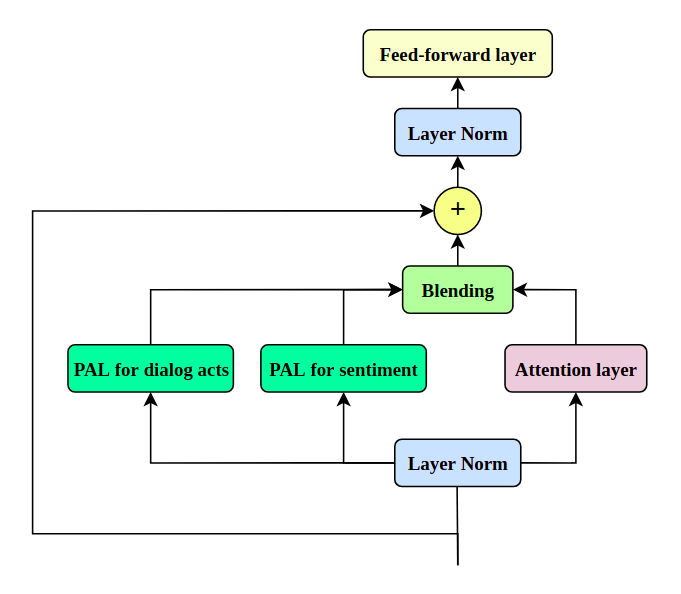
\includegraphics[width=0.7\textwidth]{img/pals_and_main.png}
%     \caption{Adding PALs to DialoGPT}
%     \label{adding_pals_dialogpt}
% \end{figure*}

% $H^{l-1}$ - output of the previous transformer layer. \par
% Layer normalization of the input:
% \begin{equation}
%     H^{l}_{LN} = LayerNorm(H^{l-1})
% \end{equation}

% Feeding the normalized input into PAL for dialog act:
% \begin{equation}
%     H^{l}_{DA} = PAL^{l}_{DA}(H^{l}_{LN})
% \end{equation}

% Feeding the normalized input into PAL for sentiment:
% \begin{equation}
%     H^{l}_{Sent} = PAL^{l}_{Sent}(H^{l}_{LN})
% \end{equation}

% Self-attention (the same as in base DialoGPT):
% \begin{equation}
%     H^{l}_{attn} = ATTN(H^{l}_{LN})
% \end{equation}

% average blending:
% \begin{equation}
%     H^{l}_{average\_blend} = \frac{1}{3}(H^{l}_{DA} + H^{l}_{Sent} + H^{l}_{attn})
% \end{equation}

% Dense blending:
% \begin{equation}
%     H^{l}_{dense\_blend} = FFN^{l}_{blend}([H^{l}_{DA}, H^{l}_{Sent}, H^{l}_{attn}])
% \end{equation}
% where [..., ...] is concatenation of several vectors.

% Combination of dense and average blending:
% \begin{equation}
%     H^{l}_{DA\_Sent} = FFN^{l}_{blend}([H^{l}_{DA}, H^{l}_{Sent}])
% \end{equation}

% \begin{equation}
%     H^{l}_{dense\_average\_blend} = \frac{1}{2}(H^{l}_{DA\_Sent} + H^{l}_{attn})
% \end{equation}
\subsection{Resources}
\label{sec:resources_consumption}
For all experiments, we used NVIDIA GeForce GTX 1080 Ti GPUs. Training DialoGPT-small with one attribute control for $10000$ steps took about $8$ hours using two GPUs. Training model with two attribute control and (weighted) average blending for $5000$ steps took about $6$ hours, with dense blending - about $8$ hours, and with a combination of average and dense blending - $7$ hours on two GPUs. Train only blend layer for a combination of dense and average took about $11$ hours on the same devices. The batch size was set to $256$ divided into $8$ steps of gradient accumulation. Extended Blenderbot was trained with batch size of 1000 on 10 NVIDIA GeForce GTX 1080 Ti GPUs. Pretraining on part of Reddit dataset (dump from 2014 and 2015 years) took 48 hours. 

%Train model with one attribute control for $10000$ steps tooks about $8$ hours using two NVIDIA GeForce GTX 1080 Ti GPUs. Batch size was set to $256$ divided on $8$ steps of gradient accumulation.

%as well as by training time the most interpreted and scalable way. Train model with (weighted) average blending for $5000$ steps took about $6$ hours, with dense blending about $8$ hours, and with combination of average and dense - $7$ hours using two NVIDIA GeForce GTX 1080 Ti GPUs. Train only blend layer for combination of dense and average took about $11$ hours on the same devices. Batch size was set to $256$ divided on $8$ steps of gradient accumulation.




\subsection{Evaluation and Classifiers}
\label{sec:eval_cls}
We used the validation part of the DailyDialog \cite{li2017dailydialog} dataset to evaluate our models. DailyDialog is labeled with dialog acts, moreover, we needed labels for the sentiment. Number of utterance for each attribute is shown on Figure \ref{dailydialog_val_da_sent_balance}. Since classes are not balanced, we used balanced accuracy (from package scikit-learn 0.21.2, sklearn.metrics.balanced\_accuracy). To evaluate the model we generated responses on the test set with the right PALs (according to the gold labels) and check if the response was generated with desired attributes. Consequently, we needed to classify dialog acts and sentiment to (1) evaluate our model and (2) label datasets automatically.

For dialog acts and sentiment classification we used the BERT-based model. One (current) or two utterances (current and previous), separated with SEP-token, were fed into BERT. The hidden state of the BERT CLS-token was fed into the dense layer, followed by softmax classification. Dialog acts classifier was trained on Daily Dialog \cite{li2017dailydialog}, sentiment classifier - on Scenario SA \cite{9091843scenario}. Balanced accuracy of dialog act classifier is $72.90\%$, the confusion matrix is in Figure \ref{da_classifier_no_hist_conf}. The balanced accuracy of the sentiment classifier is $76.24\%$.

% TODO: sentiment classifier balanced accuracy & confusion matrix

\begin{figure*}
    \centering
    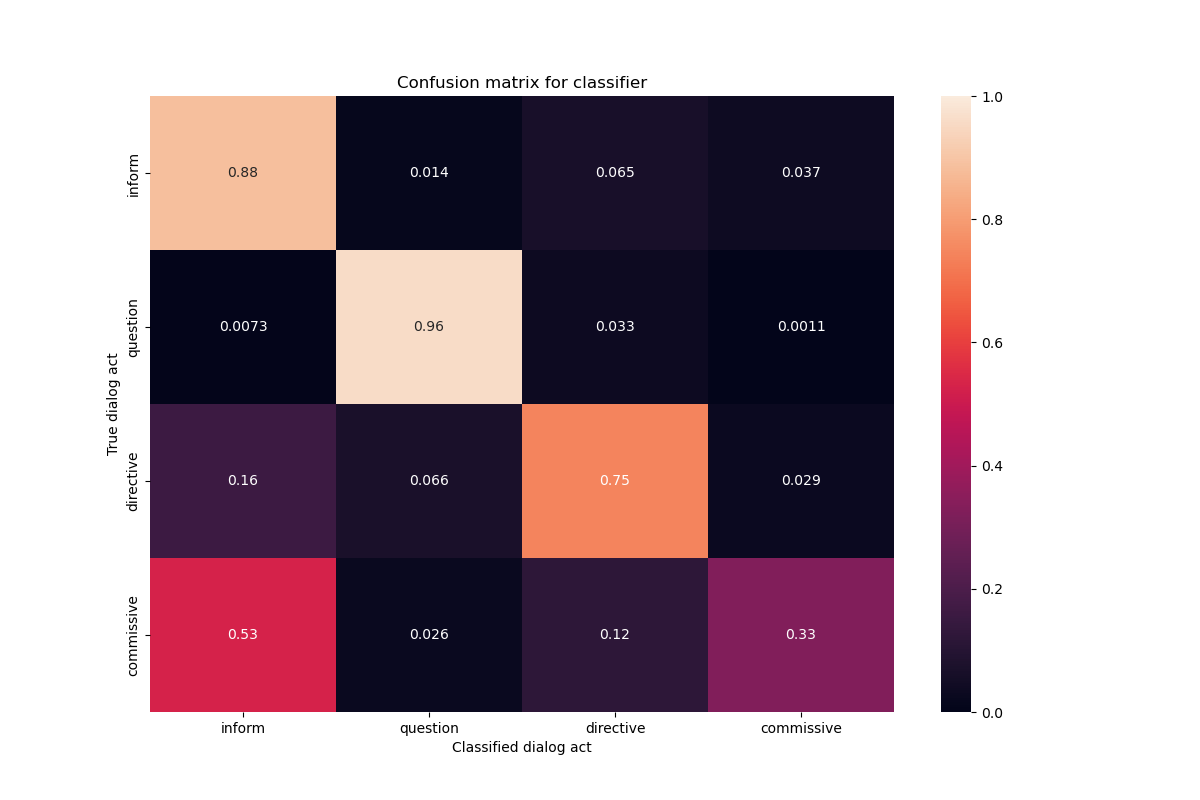
\includegraphics[scale=0.5]{img/da_classifier_conf_no_hist.png}
    \caption{Confusion matrix for dialog acts classifier.}
    \label{da_classifier_no_hist_conf}
\end{figure*}

\begin{figure*}
    \centering
    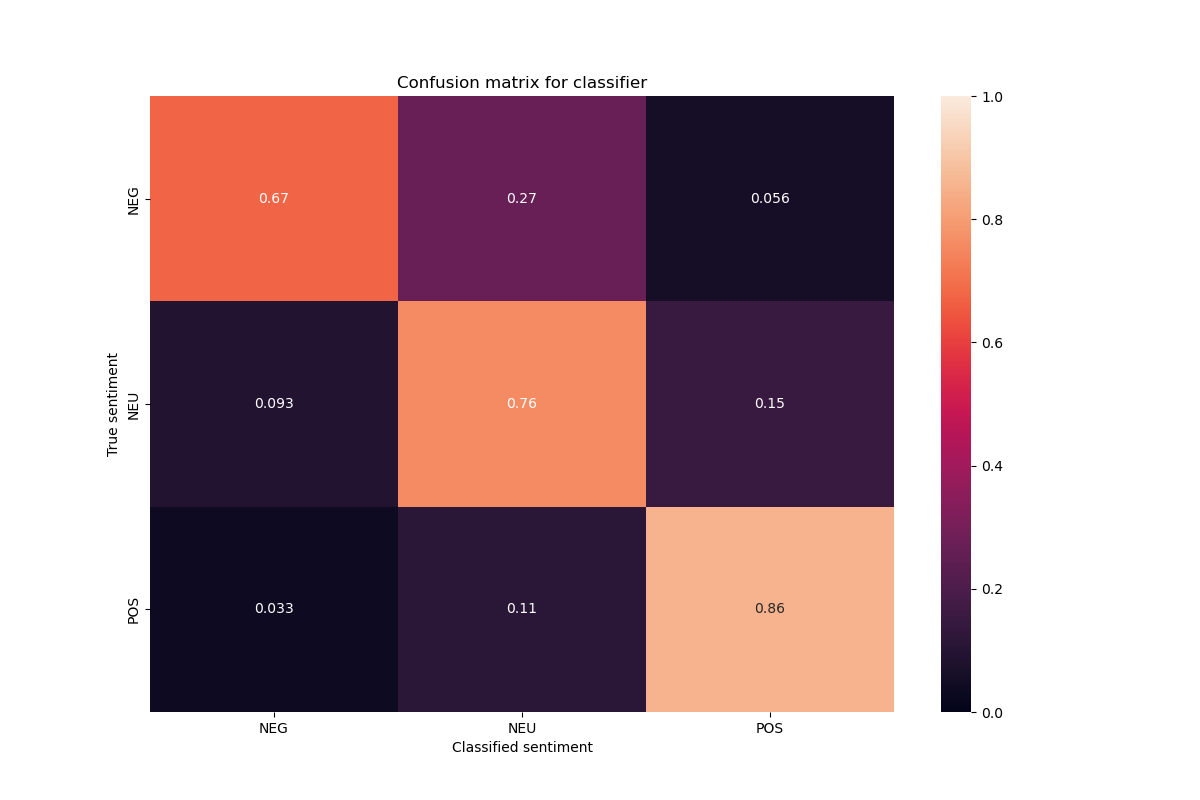
\includegraphics[scale=0.5]{img/sent_classifier_conf.png}
    \caption{Confusion matrix for sentiment classifier.}
    \label{sent_classifier_conf}
\end{figure*}

\begin{figure*}
    \begin{tabular}{cccc}
    \subfloat[Dialog acts balance]{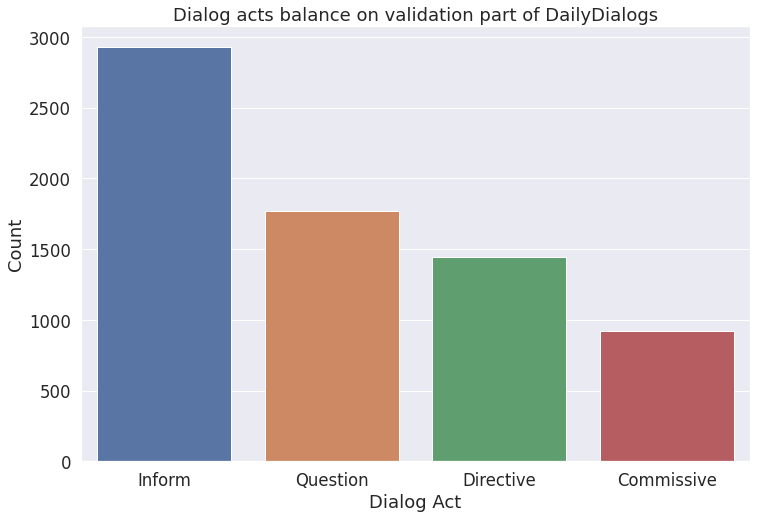
\includegraphics[width = 2.8in]{img/dailydialog_da_balance.png}} &
    \subfloat[Sentiment balance]{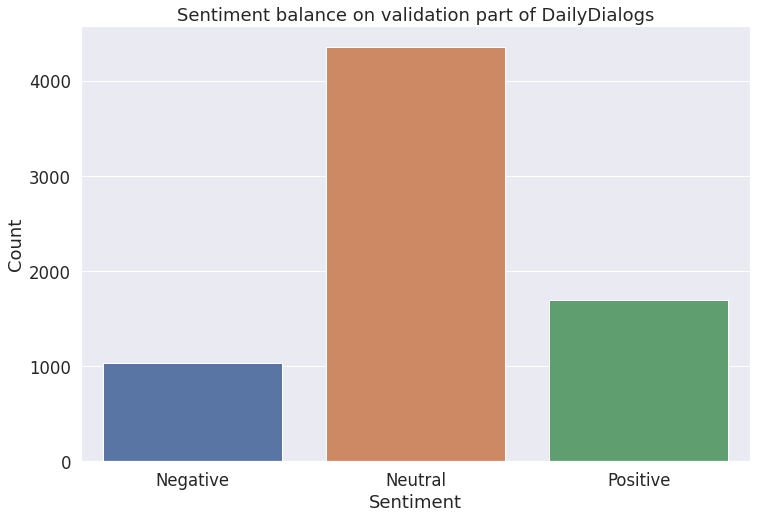
\includegraphics[width = 2.8in]{img/dailydialog_sent_balance.png}} \\
    \end{tabular}
    \caption{Attributes balance on validation set of DailyDialog}
    \centering
    \label{dailydialog_val_da_sent_balance}
\end{figure*}

\subsection{Default branch}
We added \textit{"default" branch} for each attribute for the cases when we don't want or don't need to control it. The default branch is the same PAL as the other, except during training it turns on every time instead of any other PAL for this attribute with the probability $p$, we chose $p = 0.2$. To check that the default branch is working as expected, we evaluated the model (DialoGPT-small with control of dialog acts and sentiment and combination of dense and average as a blend layer) in four setups: 
\begin{itemize}
    \item Usual inference (default branch is off)
    \item Default branch is always set for dialog act attribute
    \item Default branch is always set for sentiment attribute
    \item Default branch is always set for both dialog act and sentiment attributes
\end{itemize}

The results are in the Table \ref{default_branches_dense_average}. With default control of each attribute is back on the level of base models (without attribute control). With default branches, perplexity grows, but not too much. That averages that those branches are trained pretty well and that our model is better at control (than base DialoGPT) not just because of the larger number of parameters, but because PALs are learning their domains. Otherwise, default branches would show great control abilities too.

\begin{table*}[ht]
\fontsize{9}{11}
\selectfont 
\centering
\begin{tabular}{cccc}
\hline
Default attributes       & Dialog act acc.  & Sentiment acc.   & Perplexity       \\ \hline
No default               & \score{62.76}{0.70} & \score{70.03}{2.04} & \bestscore{15.69}{0.19} \\
Dialog act               & \score{31.97}{0.42} & \bestscore{70.19}{2.27} & \score{16.34}{0.28} \\
Sentiment                & \bestscore{62.85}{0.38} & \score{42.47}{0.75} & \score{16.03}{0.17} \\
Dialog act and sentiment & \score{30.06}{0.79} & \score{39.67}{0.31} & \score{16.83}{0.57} \\ \hline
\end{tabular}
\caption{Work of default branches for each attribute. Evaluated with the model for dialog act and sentiment control with a combination of dense and average blending.}
\label{default_branches_dense_average}
\end{table*}

\subsection{Average and weighted average blending}
\label{sec:average_blending}
Originally \cite{stickland2019bert} the output of PALs is added to the output of the corresponding layer in the base model. But we run several PALs simultaneously. We can still just add all PAL's outputs to hidden states of the main model, but since we add an arbitrary number of PALs in parallel, the summation scales poorly. This is due to the inconsistency of absolute values of hidden states and their dependency on the number of attributes to control. For this reason, we choose average as a blending layer. Since there are no trainable parameters on the blending stage, each PAL output is an embedding, shifted in a proper direction in the latent space. Furthermore, we can easily transfer the weights of PALs from a model for one-attribute control to a model with the control of several attributes. But average blending with one attribute has the following formula:
\begin{equation}
Emb = \frac{Main + PAL}{2}
\end{equation}

Average blending for several attributes has the following formula:

\begin{equation}
Emb = \frac{Main + PAL_1 + \dots + PAL_N}{N + 1}
\end{equation}

If we transfer weights with an average blending layer then each PAL would influence more than it was in a model with a single attribute control. For example with two attributes:

\begin{equation}
    Emb = \frac{Main + PAL_1 + PAL_2}{3} = \frac{1}{2}\left(\frac{Main + 2 \cdot PAL_1}{3} + \frac{Main + 2 \cdot PAL_2}{3}\right)
\end{equation}

For this reason, control abilities may be better, but perplexity will probably drop. To solve this problem we tried weighted average:
\begin{equation}
    Emb = \frac{N \cdot Main + PAL_1 + \dots + PAL_N}{2N}
\end{equation}
For two attributes is:
\begin{equation}
    Emb = \frac{2 \cdot Main + PAL_1 + PAL_2}{4}
\end{equation}
In our experiments weighted averaging significantly improved perplexity and dropped accuracy a little (Table \ref{two_attributes_control}). 

In the same way, we can directly control, how much each attribute influences the resulting embedding by tuning the weights for each attribute branch. For example, we can add more weight to dialog act PAL and get better accuracy for this attribute, but for other attributes, control ability will probably drop. We experimented with three models (each one controls dialog act and sentiment):
\begin{enumerate}
    \item PALs weights transferred from models with control of only one attribute without further training (Table \ref{reweighting_just_transfered})
    \item PALs weights transferred and model was trained (with weighted average blend) (Table \ref{reweighting_transfered_finetuned})
    \item Model was trained (with average blend) without transfer (Table \ref{reweighting_no_transfer})
\end{enumerate}

Visual results can be found in Figure \ref{reweighting_pals}. Results show that with and without weights transfer branches are learning desired attributes as expected, and it is possible to control the impact of each attribute if needed.

\begin{table*}[ht]
\fontsize{9}{11}
\selectfont 
\centering
\begin{tabular}{cccccc}
\hline
\multicolumn{3}{c}{Branch weights} & Dialog act & Sentiment & Perplexity \\
Dialog act   & Sentiment & Main  & acc.       & acc.      &            \\ \hline
0.33          & 0.33       & 0.33   & 57.88\%    & 62.15\%   & 44.53      \\
0.25          & 0.25       & 0.50   & 55.06\%    & 59.86\%   & 24.91      \\
0.20          & 0.20       & 0.60   & 49.81\%    & 55.66\%   & 21.89      \\ \hline
0.33          & 0.17       & 0.50   & 58.37\%    & 53.39\%   & 19.42      \\
0.38          & 0.12       & 0.50   & \textbf{60.90\%}    & 50.32\%   & \textbf{17.97}      \\
0.40          & 0.20       & 0.40   & 60.60\%    & 54.70\%   & 23.48      \\ \hline
0.17          & 0.33       & 0.50   & 49.34\%    & 64.40\%   & 36.20      \\
0.12          & 0.38       & 0.50   & 46.95\%    & \textbf{68.44\%}   & 45.67      \\
0.20          & 0.40       & 0.40   & 52.27\%    & 67.94\%   & 55.51      \\\hline
\end{tabular}
\caption{Reweighting the impact of just transferred PALs to improve control for selected attributes. Perplexity is high when the weight of sentiment PALs is high because the model for sentiment control was trained on a different dataset.}
\label{reweighting_just_transfered}
\end{table*}

\begin{table*}[ht]
\fontsize{9}{11}
\selectfont 
\centering
\begin{tabular}{cccccc}
\hline
\multicolumn{3}{c}{Branch weights} & Dialog act & Sentiment & Perplexity \\
Dialog act   & Sentiment & Main  & acc.       & acc.      &            \\ \hline
0.33          & 0.33       & 0.33   & 62.21\%    & 65.40\%   & 25.04      \\
0.25          & 0.25       & 0.50   & 64.42\%    & 68.53\%   & 15.55      \\
0.20          & 0.20       & 0.60   & 58.00\%    & 65.60\%   & \textbf{15.48}      \\ \hline
0.33          & 0.17       & 0.50   & 67.02\%    & 59.02\%   & 17.63      \\
0.38          & 0.12       & 0.50   & \textbf{67.13\%}    & 53.61\%   & 20.18      \\
0.40          & 0.20       & 0.40   & 61.52\%    & 56.18\%   & 25.97      \\ \hline
0.17          & 0.33       & 0.50   & 53.23\%    & 73.54\%   & 16.32      \\
0.12          & 0.38       & 0.50   & 46.97\%    & 74.17\%   & 17.90      \\ 
0.20          & 0.40       & 0.40   & 54.99\%    & \textbf{75.96\%}   & 18.71      \\ \hline
\end{tabular}
\caption{Reweighting the impact of transferred and finetuned PALs to improve control for selected attributes.}
\label{reweighting_transfered_finetuned}
\end{table*}

\begin{table*}[ht]
\fontsize{9}{11}
\selectfont 
\centering
\begin{tabular}{cccccc}
\hline
\multicolumn{3}{c}{Branch weights} & Dialog act & Sentiment & Perplexity \\
Dialog act   & Sentiment & Main  & acc.       & acc.      &            \\ \hline
0.33          & 0.33       & 0.33   & 65.87\%    & 69.44\%   & \textbf{16.63}      \\
0.25          & 0.25       & 0.50   & 54.08\%    & 63.84\%   & 17.37      \\
0.20          & 0.20       & 0.60   & 49.25\%    & 55.87\%   & 19.63      \\ \hline
0.33          & 0.17       & 0.50   & 61.26\%    & 54.81\%   & 18.26      \\
0.38          & 0.12       & 0.50   & 62.34\%    & 52.30\%   & 19.80      \\
0.40          & 0.20       & 0.40   & 68.27\%    & 57.56\%   & 18.24      \\
0.50          & 0.25       & 0.25   & \textbf{72.69\%}    & 59.07\%   & 25.33      \\
\hline
0.17          & 0.33       & 0.50   & 47.52\%    & 69.07\%   & 17.83      \\
0.12          & 0.38       & 0.50   & 43.23\%    & 71.39\%   & 18.58      \\ 
0.20          & 0.40       & 0.40   & 54.30\%    & 75.19\%   & 18.24      \\
0.25          & 0.50       & 0.25   & 49.67\%    & \textbf{76.52\%} & 33.46 \\
\hline
\end{tabular}
\caption{Reweighting the impact of trained together from scratch PALs to improve control for selected attributes.}
\label{reweighting_no_transfer}
\end{table*}


\begin{figure*}[ht]
    \centering
    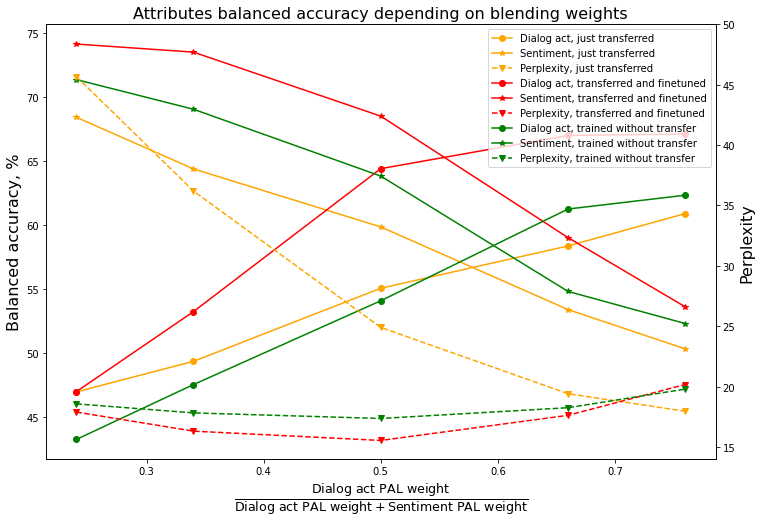
\includegraphics[scale=0.5]{img/reweighting_pals.png}
    \caption{Attributes balanced accuracy and model perplexity depending on blending weights proportion of PAL for dialog act and PAL for sentiment. Perplexity is high for a model with high sentiment impact and just transferred weights because PALs for sentiment control were trained on a different dataset.}
    \label{reweighting_pals}
\end{figure*}

\begin{figure*}[h!]
    \begin{tabular}{cccc}
    \subfloat[Pretraining of PALs, dialog acts]{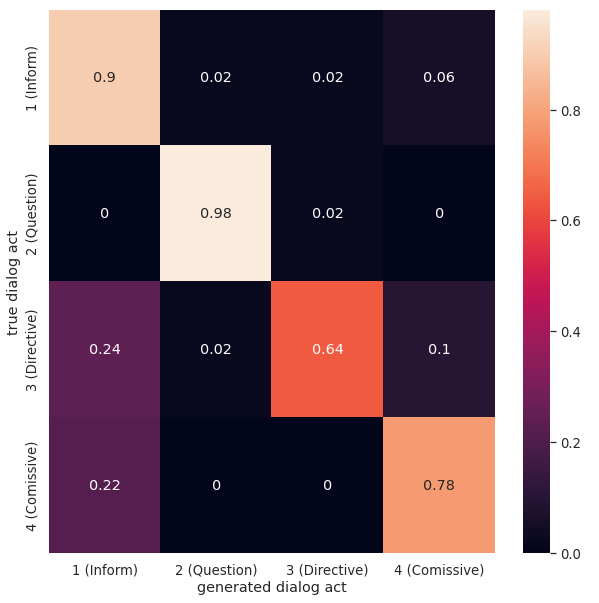
\includegraphics[width = 2.8in]{img/pals_pretrain_da.png}} &
    \subfloat[Pretraining of PALs, sentiment]{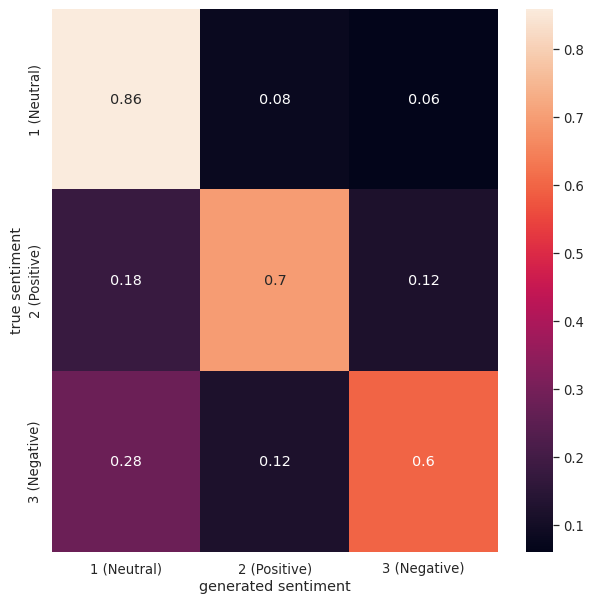
\includegraphics[width = 2.8in]{img/pals_pretrain_sent.png}} \\
    \subfloat[Fine-tuning of PALs, dialog acts]{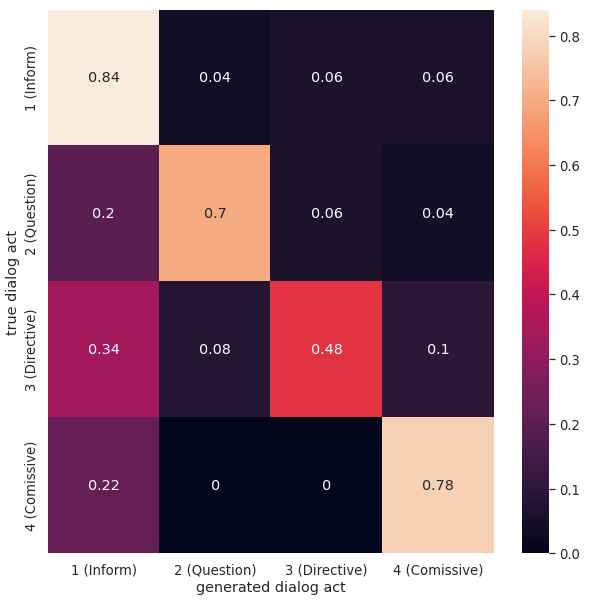
\includegraphics[width = 2.8in]{img/pals_finetune_da.png}} &
    \subfloat[Fine-tuning of PALs, sentiment]{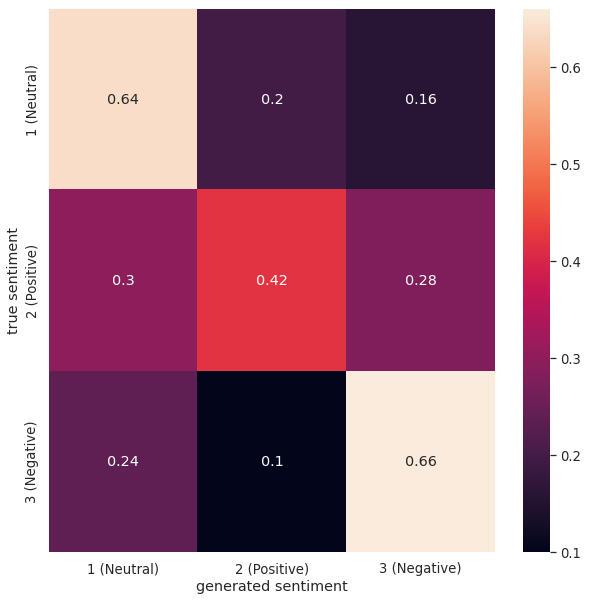
\includegraphics[width = 2.8in]{img/pals_finetune_sent.png}}\\
    \subfloat[Different attributes in batch, dialog acts]{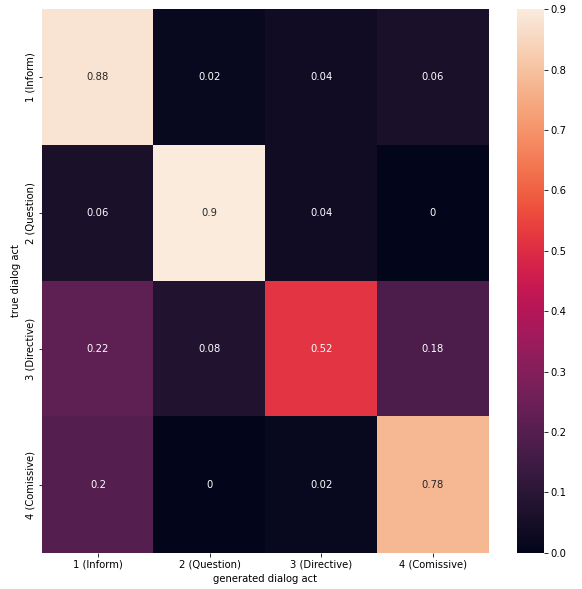
\includegraphics[width = 2.8in]{img/segm_pals_da.png}} &
    \subfloat[Different attributes in batch, sentiment]{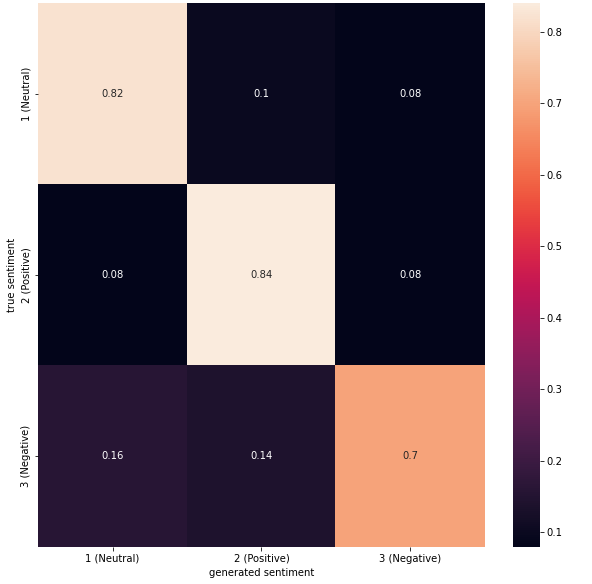
\includegraphics[width = 2.8in]{img/segm_pals_sent.png}}
    \end{tabular}
    \caption{Comparison of different training methods}
    \label{compare_training_methods}
\end{figure*}

\subsection{Comparison of pretraining and fine-tuning}
\label{sec:comp_pretrain_and_finetune}

We trained different architectures and methods of pretraining on OpenSubtitles dataset and then evaluated them on the test set of Daily Dialog. Samples from OpenSubtitles were preprocessed with classifiers for dialog acts and sentiment. We left only samples with the confidence of dialog act classification upper 0.5 and sentiment upper 0.8, in total, the dataset contains 8.9M samples. \par

To run the experiments faster, we used a very small version of DialoGPT with 6 layers and embedding dimension 256. The Table~\ref{tab:com_small_models} shows a comparison for small models. We compared the following cases:
\begin{enumerate}
     \item PALs added at every layer of DialoGPT in place of the main branch, the PALs are pre-trained at the same time as the model;
     \item PALs added in parallel with the main branch, the model is first pre-trained without PALs and then froze with only PALs training;
     \item PALs in place of the main branch and at training the batch contains samples for different dialog acts and sentiments.
\end{enumerate} \par

Pretraining of PALs results in higher accuracy of attribute generation than fine-tuning.

\begin{table*}[ht]
\fontsize{9}{11}
\selectfont 
\centering
\begin{tabular}{lccc}
\hline
Training setting          & Dialog acts accuracy & Sentiment accuracy & \multicolumn{1}{l}{Perplexity} \\ \hline
PALs, pretraining with the main model         & \score{78.73}{0.86}                 & \score{71.20}{1.91}               & \bestscore{315.06}{3.11}                           \\ %\hline
PALs, freezed main model          & \score{70.50}{2.62}                 & \score{62.07}{3.27}               & \score{368.54}{8.97}                           \\ %\hline
PALs, different attributes in batch & \bestscore{80.32}{2.79}                 & \bestscore{74.13}{3.43}                 & \score{365.60}{11.50}                           \\ \hline
\end{tabular}
\caption{Comparison of PALs training methods on small DialoGPT}
\label{tab:com_small_models}
\end{table*}


\subsection{Blenderbot evaluation}
\label{sec:blenderbot_evaluation}
We pre-train Blenderbot on Reddit and finetuned on Daily Dialog, ConvAI2, Empathetic Dialogue, and Wizard of Wikipedia.
For testing on Wizard of Wikipedia, we left in the dataset only samples with "checked sentence"{} (gold grounding knowledge).

\subsection{Perplexity-accuracy tradeoff}
\label{sec:perplexity_accuracy_tradeoff}
From one point of view, by telling the model the exact values of some attributes we giving more information and making it easier to give more value to a correct answer, so perplexity should drop. Also, by adding adapters we add more weights making the model potentially stronger. But from the other side, we have a relatively small dataset for a model to understand attributes perfectly, moreover, in our setup each adapter is trained only on part of a dataset, corresponding to its attribute value. If there isn't much data, the model will easily overfit (memorize some answers) and the control accuracy score will be high, so as perplexity because the model will have more confidence in memorized answers, we don't want this to happen. For this reason, we may not want to fine-tune the entire model and are trying to keep its output significant on each layer (averaging adapters with a fixed weight of the main branch during blending, so the model can't ignore outputs from this branch). Experiments in Appendix \ref{sec:average_blending}, Table \ref{reweighting_just_transfered}, \ref{reweighting_transfered_finetuned} show that increasing the main branch's blending weight often improves (lowers) perplexity, given that the main branch was not trained on this dataset, which means that initial language model carries important knowledge and pays attention to the dialog flow. From dialogs \ref{tab:cake_example_dialog}, \ref{tab:tea_example_dialog} we can see, that model can incorporate desired attributes in context-related answers (not just a safe universal answers), which are unlikely presented in the training dataset.

\subsection{Ethical Considerations}
\label{sec:ethical_considerations}
Generative models are known for their ability to produce offensive content of any kind. We haven't done any additional filtering of datasets we use, and the initial models (DialoGPT, Blenderbot) also have issues with producing potentially harmful content. Also in this work we control sentiment. For positive sentiment generation may be more polite, while for the negative sentiment toxicity and offence may appear more often. It's important to say, that our approach is aimed to guide model in desired direction, not to stop it from generating in undesired one.

\subsection{Dialog examples}
\label{sec:dialog_examples}

We providing some examples of dialogs with DialoGPT-small as an initial model and weighted average blending for dialog act and sentiment PALs. In Example \ref{tab:example_pos_question_dialog} positive sentiment and question dialog act was set for the whole dialog, in Example \ref{tab:example_neg_inform_dialog} - negative sentiment and inform dialog act, and in Example \ref{tab:example_pos_direct_dialog} - positive sentiment and direct dialog act. In other examples (\ref{tab:soup_example_dialog}, \ref{tab:tea_example_dialog}, \ref{tab:cake_example_dialog}) attributes were set dynamically before each system turn. Model follows desired direction in terms of attributes, but often ignores context and contradict itself. It is not an unexpected behaviour, since these problems are present in DialoGPT itself.

Sentiment control sometimes goes with emotional expressions (\textit{"Wow!"}, \textit{"How exciting!"}, or see Example \ref{tab:example_pos_question_dialog}), but the attitude of the whole utterance is also affected by selected sentiment. Inform and question dialog acts are the most popular and not so hard to master - they don't require deep semantic understanding, and model is good at asking questions and giving information (Examples \ref{tab:example_pos_question_dialog}, \ref{tab:example_neg_inform_dialog}). But directive dialog act requires a bit more analysis (classifier also has problems with direct dialog act, see Appendix \ref{sec:eval_cls}), and model catches it too (see Examples \ref{tab:example_pos_direct_dialog}, \ref{tab:soup_example_dialog}, \ref{tab:tea_example_dialog}). 

\begin{table}[]
\begin{tabular}{rl}
\multicolumn{1}{c}{Speaker}   & \multicolumn{1}{c}{Utterance}                 \\ \hline
\textbf{USER}:                         & Hello!                                        \\
\textbf{BOT} \textit{{[}Question, Positive{]}}: & Hi ! What a great moment . What's up ?        \\
\textbf{USER}:                         & Actually nothing, just want to talk.          \\
\textbf{BOT} \textit{{[}Question, Positive{]}}: & What happened ?                               \\
\textbf{USER}:                         & It's rainy...                                 \\
\textbf{BOT} \textit{{[}Question, Positive{]}}: & How are you today ?                           \\
\textbf{USER}:                         & Pretty well                                   \\
\textbf{BOT} \textit{{[}Question, Positive{]}}: & Great ! Do you like the rain ?                \\
\textbf{USER}:                         & Yes, I really love it.                        \\
\textbf{BOT} \textit{{[}Question, Positive{]}}: & What's the matter ?                           \\
\textbf{USER}:                         & Nothing)                                      \\
\textbf{BOT} \textit{{[}Question, Positive{]}}: & Oh , how exciting ! How's the weather today ?
\end{tabular}
\caption{Example of dialog with small DialoGPT model and PALs for sentiment and dialog act control, blended with a weighted average. Positive sentiment and question dialog act were set for the entire conversation.}
\label{tab:example_pos_question_dialog}
\end{table}


\begin{table}[]
\begin{tabular}{rl}
\multicolumn{1}{c}{Speaker} & \multicolumn{1}{c}{Utterance}                                                                                                              \\ \hline
\textbf{USER}:                       & Hello!                                                                                                                                     \\
\textbf{BOT} \textit{{[}Inform, Negative{]}}: & Hi , I am George .                                                                                                                         \\
\textbf{USER}:                       & Can we meet?                                                                                                                               \\
\textbf{BOT} \textit{{[}Inform, Negative{]}}: & I'm afraid that I can't meet you .                                                                                                         \\
\textbf{USER}:                       & Why? Are you busy?                                                                                                                         \\
\textbf{BOT} \textit{{[}Inform, Negative{]}}: & No , I'm afraid I'm not .                                                                                                                  \\
\textbf{USER}:                       & So what happened?                                                                                                                          \\
\textbf{BOT} \textit{{[}Inform, Negative{]}}: & \begin{tabular}[c]{@{}l@{}}My dad told me that I was going to move to Europe , \\ and he wasn't on the phone anymore .\end{tabular}        \\
\textbf{USER}:                       & Is your dad lost??? What happened?                                                                                                         \\
\textbf{BOT} \textit{{[}Inform, Negative{]}}: & \begin{tabular}[c]{@{}l@{}}He just dropped me off in the middle of the street \\ and told me he was going to move to Europe .\end{tabular} \\
\textbf{USER}:                       & \begin{tabular}[c]{@{}l@{}}So you are not going to move to Europe? \\ Do you have any troubles here?\end{tabular}                          \\
\textbf{BOT} \textit{{[}Inform, Negative{]}}: & No .                                                                                                                                      
\end{tabular}
\caption{Example of dialog with small DialoGPT model and PALs for sentiment and dialog act control, blended with a weighted average. Negative sentiment and inform dialog act were set for the entire conversation.}
\label{tab:example_neg_inform_dialog}
\end{table}

\begin{table}[]
\begin{tabular}{rl}
\multicolumn{1}{c}{Speaker}    & \multicolumn{1}{c}{Utterance}                                                             \\ \hline
\textbf{USER}:                          & Hello!                                                                                    \\
\textbf{BOT} \textit{{[}Directive, Positive{]}}: & \begin{tabular}[c]{@{}l@{}}Hello again , I'm afraid I've been here too long . \\ I need to check your homework for me .\end{tabular} \\
\textbf{USER}:                          & Okay, I've done it yesterday. Take a look.                                                \\
\textbf{BOT} \textit{{[}Directive, Positive{]}}: & I'm glad I did . Now do my homework .                                                     \\
\textbf{USER}:                          & \begin{tabular}[c]{@{}l@{}}Oh, that's a bit confusing. Don't you think, \\that homework should be done by you? \end{tabular}          \\
\textbf{BOT} \textit{{[}Directive, Positive{]}}: & \begin{tabular}[c]{@{}l@{}} I think so.I think I will write it out myself. \\ If you need a hand on it , ask me .\end{tabular}         \\
\textbf{USER}:                          & \begin{tabular}[c]{@{}l@{}}That's a good news! Actually, \\ I need you to help me with my computer.\end{tabular}                     \\
\textbf{BOT} \textit{{[}Directive, Positive{]}}: & Let's try again .                                                                         \\
\textbf{USER}:                          & What should we try again?                                                                 \\
\textbf{BOT} \textit{{[}Directive, Positive{]}}: & Just tell me again .                                                                      \\
\textbf{USER}:                          & I need you to help me with my computer.                                                   \\
\textbf{BOT} \textit{{[}Directive, Positive{]}}: & thank you .                                                                              
\end{tabular}
\caption{Example of dialog with small DialoGPT model and PALs for sentiment and dialog act control, blended with a weighted average. Positive sentiment and direct dialog act were set for the entire conversation.}
\label{tab:example_pos_direct_dialog}
\end{table}

\begin{table}[]
\begin{tabular}{rl}
\multicolumn{1}{c}{Speaker}    & \multicolumn{1}{c}{Utterance}                                                                 \\ \hline
\textbf{USER}:                          & Hello!                                                                                        \\
\textbf{BOT} \textit{{[}Inform, Positive{]}}:    & Hello ! I am glad to hear that you like our soup !                                            \\
\textbf{USER}:                          & Oh, actually I haven't said anything, but I really liked your soup!                           \\
\textbf{BOT} \textit{{[}Question, Positive{]}}:  & Soup ? I love soup .                                                                          \\
\textbf{USER}:                          & Oh, okay..                                                                                    \\
\textbf{BOT} \textit{{[}Directive, Positive{]}}: & \begin{tabular}[c]{@{}l@{}}I love soup ! It's full of flavour and it's healthy ! \\ Can you give it some fresh banana too ?\end{tabular}
\end{tabular}
\caption{Example of dialog with small DialoGPT model and PALs for sentiment and dialog act control, blended with a weighted average. Sentiment and dialog act for bot response were selected before each bot's turn.}
\label{tab:soup_example_dialog}
\end{table}

\begin{table}[]
\begin{tabular}{rl}
\multicolumn{1}{c}{Speaker}    & \multicolumn{1}{c}{Utterance}                                            \\ \hline
\textbf{USER}:                          & Do you want a cup of tea?                                                \\
\textbf{BOT} \textit{{[}Question, Positive{]}}:  & Yes , of course . Do you have a large teethen tea ?                      \\
\textbf{USER}:                          & I'm afraid no, but we will serve you our best one!                       \\
\textbf{BOT} \textit{{[}Directive, Positive{]}}: & Good , I will take the tea for free .                                    \\
\textbf{USER}:                          & Oh, yes, of course                                                       \\
\textbf{BOT} \textit{{[}Question, Positive{]}}:  & That sounds really good . But , don't you want some tea ?                \\
\textbf{USER}:                          & Yes, I will make one for myself too                                      \\
\textbf{BOT} \textit{{[}Directive, Positive{]}}: & Please do tell me when you arrive . I'll send the tea gift card to you . \\
\textbf{USER}:                          & Oh, thank you! How is it going?                                          \\
\textbf{BOT} \textit{{[}Inform, Negative{]}}:    & You look like you're leaving .                                           \\
\textbf{USER}:                          & No, I'm listening to you carefully.                                      \\
\textbf{BOT} \textit{{[}Inform, Positive{]}}:    & No problem . I'm sorry . Thanks to you , bye !                          
\end{tabular}
\caption{Example of dialog with small DialoGPT model and PALs for sentiment and dialog act control, blended with a weighted average. Sentiment and dialog act for bot response were selected before each bot's turn.}
\label{tab:tea_example_dialog}
\end{table}

\begin{table}[]
\begin{tabular}{rl}
\multicolumn{1}{c}{Speaker}    & \multicolumn{1}{c}{Utterance}                               \\ \hline
\textbf{USER}:                          & What did you eat today?                                     \\
\textbf{BOT} \textit{{[}Inform, Positive{]}}:    & I ate a turkey leg and a banana .                           \\
\textbf{USER}:                          & Was it yummy?                                               \\
\textbf{BOT} \textit{{[}Inform, Negative{]}}:    & It wasn't good , but my stomach was horrible .              \\
\textbf{USER}:                          & I'm so sorry.                                               \\
\textbf{BOT} \textit{{[}Question, Negative{]}}:  & What did you do ?                                           \\
\textbf{USER}:                          & I made and ate a cake!                                      \\
\textbf{BOT} \textit{{[}Question, Positive{]}}:  & Wow ! What did you make ?                                   \\
\textbf{USER}:                          & I made a cheesecake.                                        \\
\textbf{BOT} \textit{{[}Directive, Positive{]}}: & I am so happy .                                             \\
\textbf{USER}:                          & I'm happy too!                                              \\
\textbf{BOT} \textit{{[}Directive, Positive{]}}: & Me too ! There's a sweet strawberry on it . You can do it !
\end{tabular}
\caption{Example of dialog with small DialoGPT model and PALs for sentiment and dialog act control, blended with a weighted average. Sentiment and dialog act for bot response were selected before each bot's turn.}
\label{tab:cake_example_dialog}
\end{table}
    

\end{document}
